\documentclass[
	% -- opções da classe memoir --
	12pt,						% tamanho da fonte
	openright,					% capítulos começam em pág ímpar (insere página vazia caso preciso)
	oneside,					% para impressão em recto e verso. Oposto a oneside
	a4paper,					% tamanho do papel. 
	% -- opções da classe abntex2 --
	%chapter=TITLE,				% títulos de capítulos convertidos em letras maiúsculas
	%section=TITLE,				% títulos de seções convertidos em letras maiúsculas
	%subsection=TITLE,			% títulos de subseções convertidos em letras maiúsculas
	%subsubsection=TITLE,		% títulos de subsubseções convertidos em letras maiúsculas
	% -- opções do pacote babel --
	english,					% idioma adicional para hifenização
	brazilian						% o último idioma é o principal do documento
	]{abntex2}

\usepackage{xltabular} % Permite tabelas com colunas X que quebram páginas
\usepackage{dsfont}
\usepackage{booktabs}  % Para comandos \toprule, \midrule e \bottomrule
\usepackage{tabularx} % Necessário no preâmbulo
\usepackage{booktabs} % Necessário no preâmbulo
\usepackage{lmodern}			% Usa a fonte Latin Modern			
\usepackage[T1]{fontenc}		% Selecao de codigos de fonte.
\usepackage[utf8]{inputenc}		% Codificacao do documento (conversão automática dos acentos)
\usepackage{indentfirst}		% Indenta o primeiro parágrafo de cada seção.
\usepackage{color}				% Controle das cores
\usepackage{graphicx}			% Inclusão de gráficos
\usepackage{microtype} 			% para melhorias de justificação
\usepackage{lipsum}				% para geração de dummy text
\usepackage[brazilian,hyperpageref]{backref}	 % Paginas com as citações na bibl
\usepackage[alf]{abntex2cite}	% Citações padrão ABNT
\usepackage{multirow}
\usepackage{colortbl}
\usepackage{xcolor}
\usepackage{pdfpages}
\usepackage{amsmath}
\usepackage{amssymb}
\usepackage{forest}
\usepackage{fontawesome}
\usepackage{booktabs}
\usepackage{array}   



\definecolor{thered}{rgb}{0.65,0.04,0.07}
\definecolor{thegreen}{rgb}{0.06,0.44,0.08}
\definecolor{thegrey}{gray}{0.5}
\definecolor{theshade}{rgb}{1,1,0.97}
\definecolor{theframe}{gray}{0.6}
\definecolor{blue}{RGB}{41,5,195} 

\usepackage{listings}
\lstset{
	basicstyle=\small, % print whole listing small
	keywordstyle=\color{blue}\bfseries, %\underbar,% underlined bold black keywords
	% keywords=[0]{uint32_t, exit},
	% keywordstyle=[0]\color{thered},
	identifierstyle=, % nothing happens
	commentstyle=\color{gray!85}, % white comments
	stringstyle=\color{thered}\ttfamily, % typewriter type for strings
	showstringspaces=false, % no special string spaces
	numbers=left,
	numberstyle=\tiny,
	stepnumber=2
}

\definecolor{folderbg}{RGB}{124,166,198}
\definecolor{folderborder}{RGB}{110,144,169}

\def\Size{4pt}
\tikzset{
  folder/.pic={
    \filldraw[draw=folderborder,top color=folderbg!50,bottom color=folderbg]
      (-1.05*\Size,0.2\Size+5pt) rectangle ++ (.75*\Size,-0.2\Size-5pt);  
    \filldraw[draw=folderborder,top color=folderbg!50,bottom color=folderbg]
      (-1.15*\Size,-\Size) rectangle (1.15*\Size,\Size);
  }
}


% Configurações do pacote backref
% Usado sem a opção hyperpageref de backref
\renewcommand{\backrefpagesname}{Citado na (s) página (s):~}
% Texto padrão antes do número das páginas
\renewcommand{\backref}{}
% Define os textos da citação
\renewcommand*{\backrefalt}[4]{
	\ifcase#1
		Nenhuma citação no texto.%
	\or%
		Citado na página #2.%
	\else
		Citado #1 vezes nas páginas #2.%
	\fi}%
\renewcommand{\orientadorname}{Docentes Responsáveis:}




%-------------------------------------------------------------------------------------
%		DADOS PESSOAIS
%		Informações básicas sobre os trabalho e os autores 
%-------------------------------------------------------------------------------------
\titulo{Reconhecimento Facial com CNN em FPGA}
\autor{}
\local{Salvador}
\data{Junho 2026}
\tipotrabalho{Trabalho Final da Disciplina} 
\tipotrabalho{Trabalho Final da Disciplina} 
\preambulo{Trabalho final da disciplina Laboratório Integrado I-A apresentado aos professores Wagner Luiz Alves de Oliveira e Edmar Egídio Purcino de Souza como requisito parcial para obtenção de nota final da disciplina.}
\orientador{Prof. Dr. Edmar Egídio Purcino de Souza \\
Prof. Dr. Wagner Luiz Alves de Oliveira
}

\instituicao{%
  Universidade Federal da Bahia - UFBA \\
  Escola Politécnica
}

%	Configurações de aparência do PDF final
\input{config_pdf}

\usepackage{float}              % Ajusta as imagens [H]

%%%%%%%%%%%%%%%%%%%%%%%%%%%%%%%%%%%%%%%%%%%%%%%%%%%%%%%%%%%%%%%%%%%%%%%%%%%%%%%%%%%%%%
%																					 %
% 							 Início do documento								     %
%																					 %
%%%%%%%%%%%%%%%%%%%%%%%%%%%%%%%%%%%%%%%%%%%%%%%%%%%%%%%%%%%%%%%%%%%%%%%%%%%%%%%%%%%%%%
\begin{document}

%\selectlanguage{english}
\selectlanguage{brazilian}

% Retira espaço extra obsoleto entre as frases.
\frenchspacing

\imprimircapa

\imprimirfolhaderosto*	% (o * indica que haverá a ficha bibliográfica)

% Inserir a lista de quadros (Nativo do abntex2)
% \pdfbookmark[0]{\listofquadrosname}{loq}
% \listofquadros*
% \cleardoublepage

% Inserir a lista de tabelas
\pdfbookmark[0]{\listtablename}{lot}
\listoftables*
\cleardoublepage%

% inserir o sumario
\pdfbookmark[0]{\contentsname}{toc}
\tableofcontents*
\cleardoublepage%


%-------------------------------------------------------------------------------------
% 		ELEMENTOS PRÉ-TEXTUAIS
%		Insire elementos pré textuais
%-------------------------------------------------------------------------------------
% ---
% RESUMOS
% ---

% resumo em português
\setlength{\absparsep}{18pt} % ajusta o espaçamento dos parágrafos do resumo
\begin{resumo}
Este trabalho apresenta o desenvolvimento de uma Fechadura Biométrica Inteligente implementada na FPGA DE2-115 (Cyclone IV EP4CE115F29C7) como projeto integrador da disciplina ENGG52 da UFBA. O sistema realiza reconhecimento facial em tempo real através de uma Rede Neural Convolucional embarcada, classificando indivíduos entre 19 classes — 18 membros autorizados e uma classe nativa de rejeição — sem necessidade de limiar de confiança externo.
A solução cobre o pipeline completo de ponta a ponta: uma câmera conectada ao PC captura o rosto do usuário, que é detectado pelo algoritmo Haar Cascade, normalizado com CLAHE, redimensionado para 32×32 pixels e transmitido via UART à placa. Na FPGA, uma Máquina de Estados Finitos orquestra o pipeline de inferência composto pelos módulos de convolução 3×3 com ReLU (4 filtros), \textit{Max Pooling} 2×2, \textit{Flatten} e camada Densa 900×19, cujos pesos foram treinados em Python com Keras, quantizados para o formato de ponto fixo Q1.7 e armazenados em blocos de memória M9K. O resultado é exibido em um monitor VGA com o nome do indivíduo reconhecido e acionamento de LEDs indicando liberação ou negação de acesso.
As validações quantitativas realizadas ao longo do projeto confirmam a fidelidade da implementação em Verilog. O sistema integra os Artefatos 1 a 4 do cronograma proposto, abrangendo aquisição e treinamento off-line, arquitetura RTL, \textit{pipeline} de visão e comunicação, e integração final.


 \textbf{Palavras-chave}: FPGA. reconhecimento facial. CNN embarcada. quantização de ponto fixo. verilog. DE2-115.
\end{resumo}



%-------------------------------------------------------------------------------------
% 		ELEMENTOS TEXTUAIS
%		Informações relevantes ao trabalho, capítulos e suas respectivas seções.
%-------------------------------------------------------------------------------------
\textual%
% Introdução
\chapter{Introdução}
O reconhecimento facial tem sido um instrumento amplamente utilizado para contextos de identificação e garantia de segurança. O mapeamento de padrões e características é essencial para o bom funcionamento de um sistema de proteção. Nesse cenário, o desenvolvimento de interfaces homem-máquina (IHM) tem avançado com o aumento da capacidade computacional em sistemas embarcados.

Para traduzir essas características em dados quantizados, as Redes Neurais Convolucionais (CNNs) têm se mostrado altamente eficazes. Em uma aplicação real voltada para a autorização da entrada de um indivíduo cadastrado em um estabelecimento, o fluxo de dados exige a aquisição de imagem em tempo real, o pré-processamento e a inferência no modelo de \textit{Deep Learning}. Contudo, a etapa de inferência impõe um alto custo computacional. Processadores de uso geral e microcontroladores processam as matrizes da rede neural de forma puramente sequencial, o que pode representar um gargalo crítico para a percepção de tempo real do usuário.

Para a implementação da rede neural no FPGA, optou-se pelo desenvolvimento manual dos módulos de \textit{hardware} utilizando a Linguagem de Descrição de \textit{Hardware} (HDL) Verilog. Essa abordagem permite maior controle sobre a arquitetura implementada, possibilitando a exploração explícita do paralelismo inerente às operações convolucionais e de multiplicação-acumulação (MAC) presentes na CNN. Além disso, a implementação manual permite avaliar de maneira mais precisa os benefícios e os custos associados ao desenvolvimento de aceleradores dedicados para aplicações de Inteligência Artificial embarcada.

\section{Objetivos}
Este trabalho tem como objetivo o desenvolvimento de uma \textit{Tiny-CNN}, seu respectivo treinamento utilizando a linguagem de programação Python através de um \textit{dataset} com fotos dos integrantes convertidas em escala cinza, a implementação de seu modelo matemático em linguagem de \textit{hardware} Verilog --- além da integração de periféricos, como o protocolo UART e a transmissão de imagem via VGA --- e o teste prático do modelo em uma placa FPGA DE2-115.

\section{Metodologia}
Os dados de treinamento foram obtidos através de uma câmera de \textit{notebook}, em sala de aula, em gravações de vídeos de cada integrante, extraindo os \textit{frames} dos vídeos utilizando a biblioteca openCV em Python e tratando-os em escala cinza e o respectivo treinamento foi realizado mediante Keras. Já o teste de funcionamento do modelo matemático em Verilog baseado na construção do modelo Python foi feito pelo \textit{software} ModelSim, e seu respectivo resultado de simulação comparado com o resultado do modelo Python.
O procedimento adotado foi a construção aditiva e gradual da rede em paralelo com implementação e testes de módulos lógicos em Verilog, orquestrados por uma Máquina de Estados Finitos (FSM) confeccionada também paralelamente.

\section{Justificativa}
O trabalho traz contribuições importantes para a literatura ao fazer um estudo comparativo do processo de inferência de redes neurais convolucionais em diferentes arquiteturas. Além disso, é capaz de atuar como referência em possíveis futuras estruturações de fluxos completos de uma CNN em um FPGA.
\nocite{Hoxha:2025:FAN}
\nocite{MADAOUI2023104927}

% Primeira Entrega
\chapter{Aquisição de Dados e Treinamento \textit{Offline}}
O foco desta etapa foi a criação de um \textit{pipeline} robusto para aquisição de dados, treinamento de uma \textit{Tiny-CNN} otimizada e a exportação dos parâmetros quantizados para o \textit{hardware}. O \textit{dataset} foi projetado para um problema de classificação multiclasse com 19 classes: Classe 0 (Desconhecidos) e Classes 1–18 (Membros autorizados).

\section{Confecção e treinamento da Rede Neural Convolucional (CNN)}

\subsection{Classes de 1 a 18: Autorizados (Equipe)}
As imagens foram extraídas de vídeos .mp4, utilizando o algoritmo Haar Cascade com scale Factor 1.2 para detecção facial, e houve a implementação do CLAHE (\textit{Contrast Limited Adaptive Histogram Equalization}) para garantir o reconhecimento sob diferentes condições de luz e sombras. Para atingir a meta de 400 imagens por integrante, houve a aplicação de técnicas de aumento de dados incluindo rotação leve (-15° a 15°), variações de zoom (0.9x a 1.1x), espelhamento horizontal e ajustes de brilho.

\subsection{Classe 0: Desconhecidos (Unknowns)}
Para minimizar falsos positivos, a Classe 0 foi expandida para garantir maior diversidade, logo tivemos a integração do LFW (\textit{Labeled Faces in the Wild}) via kagglehub e do UCF \textit{Selfie-dataset}, utilizando de uma proporção de 5:1 (Desconhecidos:Autorizados) para cobrir a variabilidade do rosto humano. Foram aplicadas então as mesmas técnicas de aumento de dados (rotação/zoom) na Classe 0 para garantir a invariância de identidade, além da inclusão de 300 imagens sintéticas (paredes e ruído) para evitar autorizações baseadas em texturas de fundo.

\begin{figure}[H]
    \centering
    \includegraphics[width=0.8\linewidth]{imagens/image6.png}
    \caption{Matriz de Confusão durante o teste}
    \label{fig1}
\end{figure}

\section{Implementação}
A rede foi projetada para ser leve (\textit{Tiny-CNN}) visando a implementação em blocos de memória M9K da FPGA, equilibrando capacidade discriminativa e custo computacional compatível com o Cyclone IV EP4CE115F29C7.
A arquitetura segue o \textit{pipeline}: Entrada 32×32 (grayscale, Q1.7) → Conv2D (4 filtros 3×3, acumuladores 20 bits) → ReLU (combinacional) → \textit{Max Pooling} 2×2 → \textit{Dropout} → \textit{Dense} (19 classes) → Softmax. 

A escolha de apenas 4 filtros convolucionais não é arbitrária — ela resulta diretamente da restrição de \textit{hardware}: cada filtro ocupa um sub-bloco M9K dedicado para armazenar seus 900 pesos densos correspondentes, e o Cyclone IV dispõe de 432 blocos M9K, dos quais 19 são consumidos pelos pesos da camada densa (um por classe) e outros são reservados para framebuffer e line buffer.

A busca de hiperparâmetros foi conduzida com \textit{Keras Tuner (Hyperband)} otimizando simultaneamente a taxa de \textit{Dropout} (0,2 a 0,5), a \textit{Learning Rate} e a regularização L2. A escolha do \textit{Hyperband} sobre o \textit{grid search} convencional foi motivada pela relação classes/parâmetros: com 19 classes e \textit{dataset} balanceado artificialmente, o espaço de hiperparâmetros relevante é estreito e o \textit{Hyperband} converge para ele com menos avaliações completas.

A regularização L2 cumpre papel duplo no projeto: além de reduzir \textit{overfitting}, ela penaliza pesos de grande magnitude durante o treino, o que reduz diretamente o erro de arredondamento introduzido pela quantização posterior para Q1.7 — pesos próximos de zero perdem menos informação relativa ao serem truncados para 8 bits do que pesos de grande amplitude.

O \textit{Custom Loss Weighting} aplicou peso 1,0 à Classe 0 (Desconhecido) e 4,0 às classes de membros autorizados (1–18), refletindo a assimetria de custo do problema: uma falsa negação — negar acesso a um membro autorizado — é operacionalmente mais custosa do que um falso positivo para a classe de rejeição. O treinamento foi conduzido com \textit{EarlyStopping} com paciência de 15 épocas, suficiente para absorver platôs de validação comuns em \textit{datasets} pequenos com \textit{augmentation} agressivo.

\begin{figure}[H]
    \centering
    \includegraphics[width=1\linewidth]{imagens/image4.png}
    \caption{Matriz de Confusão durante o teste}
    \label{fig2}
\end{figure}

\section{Inferência e Validação}
O sistema utiliza um script de validação (\texttt{inference\_webcam.py}) para testagem do desempenho do modelo treinado. Aplica-se o mesmo pré-processamento (CLAHE, Padding de 15\%, Redimensionamento) utilizado no treino, e ocorre então a exibição da ``Visão da CNN'' (32x32) para validação de qualidade com entradas em tempo real. Este fluxo ocorre completamente em \textit{software}.

\subsection{Métricas de Teste e Relatório de Classificação}

Os resultados da avaliação multiclasse durante o teste são dados a seguir:

\begin{table}[H]
\caption{Métricas de Teste}
\centering
\label{tab:metricas_modelo}
\renewcommand{\arraystretch}{1.2} % Dá um leve respiro entre as linhas
\begin{tabular}{l c}
\toprule
\textbf{Métrica} & \textbf{Valor} \\
\midrule
AUC OvR (macro)                               & 0,9999 \\
Macro-F1                                      & 0,9901 \\
Balanced Accuracy                             & 0,9918 \\
Recall da classe desconhecido (negar invasor) & 0,9608 \\
Recall macro dos alunos autorizados           & 0,9936 \\
\bottomrule
\end{tabular}
\end{table}

A Tabela \ref{tab:relatorio_classificacao} detalha as métricas de precisão, revocação (\textit{recall}) e pontuação F1 para cada classe individualmente, bem como as médias globais do sistema.

\begin{table}[H]
\centering
\caption{Relatório de Classificação do Teste}
\label{tab:relatorio_classificacao}
\begin{tabular}{l c c c c}
\toprule
\textbf{Classe} & \textbf{Precision} & \textbf{Recall} & \textbf{F1-score} & \textbf{Support} \\
\midrule
0\_desconhecido    & 0.98 & 0.96 & 0.97 & 1020 \\
10\_Igor           & 0.99 & 1.00 & 1.00 & 300  \\
11\_Joao           & 1.00 & 1.00 & 1.00 & 300  \\
12\_Jose\_Henrique & 1.00 & 1.00 & 1.00 & 119  \\
13\_Julia          & 1.00 & 1.00 & 1.00 & 300  \\
14\_Lucio          & 1.00 & 0.99 & 1.00 & 300  \\
15\_Naira          & 1.00 & 1.00 & 1.00 & 300  \\
16\_Rafael         & 0.88 & 0.93 & 0.90 & 179  \\
17\_Samuel         & 1.00 & 1.00 & 1.00 & 300  \\
18\_Yuri           & 0.98 & 1.00 & 0.99 & 300  \\
1\_Anna\_Carol     & 1.00 & 0.98 & 0.99 & 300  \\
2\_Bruno           & 1.00 & 1.00 & 1.00 & 300  \\
3\_Diego           & 0.99 & 1.00 & 1.00 & 300  \\
4\_Eduardo         & 0.97 & 1.00 & 0.99 & 300  \\
5\_Fabio           & 1.00 & 1.00 & 1.00 & 300  \\
6\_Felipe          & 1.00 & 0.99 & 1.00 & 300  \\
7\_Gabriel         & 1.00 & 1.00 & 1.00 & 300  \\
8\_Horacio         & 0.99 & 1.00 & 1.00 & 300  \\
9\_Hugo            & 0.99 & 1.00 & 1.00 & 300  \\
\midrule
\textbf{accuracy}     &      &      & 0.99 & 6118 \\
\textbf{macro avg}    & 0.99 & 0.99 & 0.99 & 6118 \\
\textbf{weighted avg} & 0.99 & 0.99 & 0.99 & 6118 \\
\bottomrule
\end{tabular}
\end{table}

\section{Quantização e Exportação (.MIF)}
Os pesos são convertidos de ponto flutuante para Ponto Fixo (Q1.7) para execução em \textit{hardware} de 8 bits, seguindo a lógica de multiplicação por 128 e arredondamento para o intervalo de -128 a 127. Então, são gerados os ficheiros .mif formatados para os blocos de memória M9K do \textit{Intel Quartus Prime}.

% ---------------------------

% Segunda Entrega
\chapter{Arquitetura de \textit{Hardware}  (RTL)}
\section{Gerenciamento de Processamento: Módulo \texttt{cnn\_top}}

O processamento da CNN é gerenciado por um módulo superior (\texttt{cnn\_top}), que instancia 9 submódulos responsáveis pela inferência da rede, coordenando-os por meio de uma Máquina de Estados Finitos (FSM) própria.

Além dos sinais oriundos dos submódulos instanciados e dos sinais básicos de \textit{clock} e \textit{reset}, o \texttt{cnn\_top} recebe três sinais externos. Dois deles vêm da lógica do controlador VGA e são utilizados na leitura do \textit{framebuffer}. O terceiro é o \textit{\textit{bit}} recebido pela comunicação serial, que passa por dois \textit{flip-flops} para mitigar problemas de metaestabilidade antes de ser enviado ao módulo UART.

As principais saídas do \texttt{cnn\_top} usadas pelo arquivo principal do projeto são detalhadas na Tabela \ref{tab:sinais_cnn_top}.

\begin{table}[htbp]
\centering
\caption{Principais saídas do módulo \texttt{cnn\_top}}
\label{tab:sinais_cnn_top}
\small
\begin{tabularx}{\textwidth}{l X}
\toprule
\textbf{Sinal} & \textbf{Descrição} \\
\midrule
\texttt{class\_id[4:0]} & Valor da classe predita (0 = Vazio, 1 = Desconhecido, 2 a 19 = Autorizados). \\
\texttt{access\_done} & Sinal que indica a finalização do processo de inferência. \\
\texttt{frame\_ready} & Sinal ativo quando o \textit{framebuffer} $32 \times 32$ está completo. \\
\texttt{frame\_mode} & Indica se a exibição será o vídeo completo ou apenas o recorte do rosto. \\
\bottomrule
\end{tabularx}
\end{table}

% TODO: Inserir diagrama das principais entradas e saídas do bloco cnn_top
\begin{figure}[H]
    \centering
    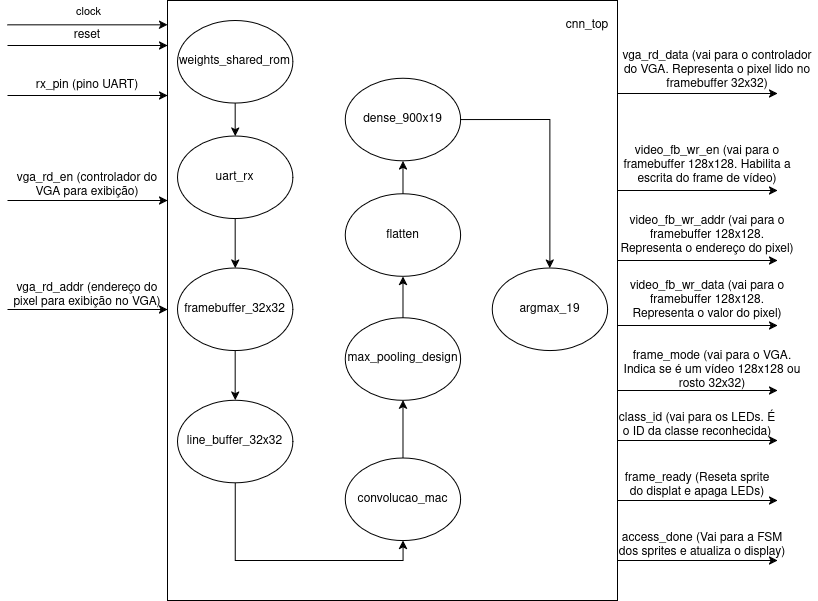
\includegraphics[width=0.7\textwidth]{imagens/image18.png}
    \caption{Diagrama de blocos das principais entradas e saídas do módulo \texttt{cnn\_top}.}
    \label{fig:diagrama_cnn_top}
\end{figure}

\subsection{Papel e Comportamento dos Submódulos}

O papel e o comportamento de cada submódulo instanciado são detalhados a seguir:

\subsubsection{UART}
Responsável pela decodificação da comunicação serial em \textit{bytes} de 8 \textit{bits}.

\begin{table}[htbp]
\centering
\caption{Principais sinais do submódulo UART}
\label{tab:sinais_uart}
\small
\begin{tabularx}{\textwidth}{l X}
\toprule
\textbf{Sinal} & \textbf{Descrição} \\
\midrule
\texttt{data\_out[7:0]} & O \textit{byte} completo montado após a recepção serial. \\
\texttt{data\_valid} & Pulso indicando que \texttt{data\_out} contém um \textit{byte} válido. \\
\bottomrule
\end{tabularx}
\end{table}

\subsubsection{\textit{Framebuffer} $32 \times 32$}
Responsável pela escrita espelhada em duas memórias internas distintas de 1024 \textit{bytes}, permitindo a leitura simultânea pela CNN e pelo módulo VGA em frequências diferentes. Durante a escrita, recebe sinais de controle e de endereço do \texttt{cnn\_top}, processando os dados advindos da UART. Na leitura da rede, a FSM do \texttt{cnn\_top} envia sinais de requisição e recebe o pixel correspondente. Para a exibição em tela, o controlador VGA faz requisições similares na segunda memória. Ao receber um sinal de \textit{reset}, todos os endereços de ambas as memórias são zerados (\texttt{0x00}).
\begin{table}[htbp]
\centering
\caption{Principais sinais do submódulo \textit{Framebuffer} $32 \times 32$}
\label{tab:sinais_framebuffer}
\small
\begin{tabularx}{\textwidth}{l X}
\toprule
\textbf{Sinal} & \textbf{Descrição} \\
\midrule
\texttt{rd\_data[7:0]} & \textit{Byte} que representa o pixel solicitado pela CNN durante a leitura do \textit{framebuffer}. \\
\texttt{frame\_ready} & Pulso que indica quando o último pixel foi armazenado durante a escrita. \\
\texttt{vga\_rd\_data[7:0]} & \textit{Byte} que representa o pixel solicitado pelo VGA durante a leitura do \textit{framebuffer}. \\
\bottomrule
\end{tabularx}
\end{table}

\subsubsection{\textit{Line Buffer}}
Durante a leitura da imagem, o módulo de \textit{Line Buffer} produz e armazena a janela $3 \times 3$ a partir do fluxo sequencial de pixels, fornecendo a matriz necessária para a convolução. Como a leitura ocorre da esquerda para a direita e de cima para baixo, o módulo retém o histórico das duas últimas linhas da imagem em blocos de memória dedicados. O deslocamento espacial para formar a janela é coordenado por sinais de controle. Ao associá-las ao pixel atual de entrada, consegue formar a saída desejada.

\begin{table}[htbp]
\centering
\caption{Principais sinais do submódulo \textit{Line Buffer}}
\label{tab:sinais_linebuffer}
\small
\begin{tabularx}{\textwidth}{l X}
\toprule
\textbf{Sinal} & \textbf{Descrição} \\
\midrule
\texttt{win[0:8][7:0]} & A ``janela'' $3 \times 3$ completa formada por cada pixel. \\
\texttt{window\_valid} & Pulso que indica a finalização da construção de uma janela válida. \\
\bottomrule
\end{tabularx}
\end{table}

\subsubsection{Convolução}
Executa a convolução 2D sobre a janela $3 \times 3$ gerada pelo \textit{Line Buffer}. Recebe os pesos e vieses dos 4 filtros quantizados em ponto fixo Q1.7. Para cada filtro, a operação de multiplicação e acumulação (MAC) segue a formulação matemática:

$$ MAC = \sum_{i} pixel(i) \cdot peso(i) + bias, \text{onde } i \in \{0, \dots, 8\} $$

Para evitar \textit{overflow} de informações, os acumuladores são operados em 20 \textit{bits} (quantizados em Q6.14). Em seguida, aplica-se a função de retificação linear (ReLU), na qual valores negativos são descartados (zerados) e valores superiores a 32767 são saturados. O resultado é truncado para 16 \textit{bits} no formato Q2.14. A cada ciclo de \textit{clock}, ele produz 4 saídas (uma por filtro):

\begin{table}[htbp]
\centering
\caption{Principais sinais do submódulo de Convolução}
\label{tab:sinais_convolucao}
\small
\begin{tabularx}{\textwidth}{l X}
\toprule
\textbf{Sinal} & \textbf{Descrição} \\
\midrule
\texttt{out\_f0} & Pixel resultante da convolução da janela com o filtro 0. \\
\texttt{out\_f1} & Pixel resultante da convolução da janela com o filtro 1. \\
\texttt{out\_f2} & Pixel resultante da convolução da janela com o filtro 2. \\
\texttt{out\_f3} & Pixel resultante da convolução da janela com o filtro 3. \\
\texttt{valid\_out} & Pulso que valida a saída da convolução. \\
\bottomrule
\end{tabularx}
\end{table}

\subsubsection{\textit{Max \textit{Pooling} }}
Possui quatro memórias para armazenar a linha anterior processada pelos 4 filtros. Por meio de um circuito combinacional, compara os quatro valores de cada sub-janela $2 \times 2$ espacial, repassando apenas o valor máximo. O módulo opera com um \textit{stride} de 2, calculando janelas apenas em coordenadas ímpares. Como gera 4 resultados simultâneos e o próximo estágio consome apenas 1 por ciclo, implementa-se um sistema FIFO de 32 posições para serializar as saídas.

\subsubsection{\textit{Flatten}  (``Achatamento'')}
Como a convolução aplicada não possui \textit{padding valid}, a imagem original $32 \times 32$ é reduzida para $30 \times 30$. Após o \textit{Pooling}, a dimensionalidade cai para $15 \times 15$ por filtro. Este módulo funciona essencialmente como um contador, serializando cada pixel recebido até atingir os 900 valores esperados ($15 \times 15 \times 4$).

\subsubsection{Camada Densa}
Responsável por realizar a classificação final. O módulo recebe cada pixel proveniente do \textit{Flatten}  e realiza o cálculo MAC com 19 pesos simultâneos (um para cada classe), acumulando os resultados ao longo dos ciclos de \textit{clock}. Quando os 900 pixels são finalizados, a camada soma os vieses. Utilizam-se acumuladores de 48 \textit{bits} para reter precisão.

\begin{table}[H]
\centering
\caption{Principais sinais do submódulo de Camada Densa}
\label{tab:sinais_camada_densa}
\small
\begin{tabularx}{\textwidth}{l X}
\toprule
\textbf{Sinal} & \textbf{Descrição} \\
\midrule
\texttt{valid\_out} & Pulso de controle que informa para o módulo seguinte que o processamento da camada densa foi concluído. \\
\texttt{done} & Pulso de controle que informa para o \texttt{cnn\_top} que o processamento da camada densa se encerrou. \\
\texttt{scores[0:18][15:0]} & 19 valores de 16 \textit{bits} formatados em Q6.10 que serão usados pelo módulo final para a inferência. \\
\bottomrule
\end{tabularx}
\end{table}

\subsubsection{Argmax}
Módulo que executa o processo final de decisão. Opera como uma FSM que varre as saídas da Camada Densa comparando os \textit{scores}. A classe correspondente ao maior valor é definida como a predição da rede. O índice gerado é internamente incrementado em 1 para se adequar à lógica do VGA, que reserva o ID 0 para a tela vazia (isto é, sem qualquer exibição de nomes).

\begin{table}[H]
\centering
\caption{Principais sinais do submódulo Argmax}
\label{tab:sinais_argmax}
\small
\begin{tabularx}{\textwidth}{l X}
\toprule
\textbf{Sinal} & \textbf{Descrição} \\
\midrule
\texttt{valid\_out} & Pulso de controle para indicar a finalização da inferência. \\
\texttt{class\_id[4:0]} & ID da classe inferida. \\
\bottomrule
\end{tabularx}
\end{table}

\subsubsection{ROM de Pesos}
Módulo responsável por ler o arquivo \texttt{.mif} de inicialização e rotear os parâmetros da rede. Ele transfere os pesos para registradores (no caso das camadas iniciais) ou blocos M9K (no caso da camada densa). Para permitir o acesso paralelo aos 19 pesos da camada densa em um único ciclo, estes são distribuídos em 19 blocos M9K individuais. Além dos parâmetros de cada camada, sua saída também inclui um \textit{bit} de controle indicando a conclusão das cópias de cada endereço.

\newpage
\noindent \textbf{Observações Importantes:}
\begin{itemize}
    \item As saídas dos módulos de \textit{Max \textit{Pooling}}  e \textit{Flatten}  são somente os pulsos de controle e o dado processado naquele bloco.
    \item A camada densa não aplica quaisquer funções de ativação. Isso ocorre por conta da lógica de escolha da saída da rede: a previsão é o ID, isto é, a posição do maior valor calculado. Importante também observar que a classe ``Desconhecido'' foi tratada como uma classe real, em contraposição à interpretação desta como a negação de todas as demais.
\end{itemize}

\subsection{Máquina de Estados de Controle}

Conhecendo os principais sinais que o \texttt{cnn\_top} gerencia, é possível descrever a FSM que controla a CNN conforme o diagrama da Figura \ref{fig:fsm_cnn} e a Tabela \ref{tab:sinais_cnn_top}.

% TODO: Inserir diagrama da FSM
\begin{figure}[H]
    \centering
    \includegraphics[width=1\textwidth]{imagens/image13.png}
    \caption{Diagrama de estados da FSM controladora da CNN no módulo \texttt{cnn\_top}.}
    \label{fig:fsm_cnn}
\end{figure}

\begin{table}[H]
\centering
\caption{Sinais de controle da FSM principal do módulo \texttt{cnn\_top}}
\label{tab:sinais_fsm_controle}
\small
\begin{tabularx}{\textwidth}{l X}
\toprule
\textbf{Sinal} & \textbf{Descrição} \\
\midrule
\texttt{argmax\_valid} & Conexão no \texttt{cnn\_top} que recebe a saída \texttt{valid\_out} do módulo Argmax. \\
\texttt{uart\_valid} & Conexão no \texttt{cnn\_top} que recebe a saída \texttt{data\_valid} do módulo UART. \\
\texttt{uart\_data} & Conexão no \texttt{cnn\_top} que recebe a saída \texttt{data\_out} do módulo UART. \\
\texttt{uart\_wr\_addr} & Sinal gerado pelo módulo \texttt{cnn\_top} durante a leitura do \textit{framebuffer}. É um contador que incrementa a cada novo \textit{byte} recebido. \\
\texttt{uart\_frame\_pending} & Sinal de controle. Enquanto a imagem está sendo lida, é 0. Sobe para 1 apenas quando \texttt{uart\_wr\_addr == 1023}. \\
\texttt{frame\_ready} & Conexão no \texttt{cnn\_top} que recebe a saída \texttt{frame\_ready} do \textit{framebuffer}. \\
\texttt{frame\_mode} & Pulso de saída que indica ao VGA se a exibição deverá ser de um rosto ou do vídeo. \\
\texttt{weights\_boot\_done} & Sinal de controle que indica que o processo de gravação de pesos foi concluído. \\
\texttt{frame\_clear} & Sinal enviado para ``desligar'' o \texttt{frame\_ready} assim que a rede inicia uma nova inferência. \\
\texttt{rd\_val\_count} & Contador que indica o progresso de leitura da memória síncrona M9K. \\
\bottomrule
\end{tabularx}
\end{table}

\section{Validação da Arquitetura de \textit{Hardware} }

Para validar as inferências em ponto fixo realizadas pelo \textit{hardware}, fez-se necessária a comparação dessas saídas com seus respectivos valores em ponto flutuante, obtidos via \textit{software}. Para tanto, considerando uma mesma imagem de entrada, adotaram-se procedimentos e métricas específicas de avaliação, estruturados da seguinte forma:

\begin{enumerate}
    \item \textbf{Seleção das Camadas:} Os valores comparados correspondem às saídas dos módulos de Convolução, \textit{Max \textit{Pooling}}, \textit{Flatten}, Camada Densa e ao resultado final da inferência.
    \item \textbf{Extração e Quantização em Software:} Cada valor foi extraído do modelo em \textit{software} e quantizado para o formato de ponto fixo equivalente ao do \textit{hardware}. Nas camadas de convolução, \textit{Pooling} e \textit{Flatten}, os valores foram multiplicados por $2^{14}$ e arredondados. Na camada densa, a saída foi calculada sem a aplicação da função de ativação (\textit{Softmax}) e, em seguida, quantizada no formato Q6.10.
    \item \textbf{Extração em \textit{Hardware} :} Os valores processados fisicamente pelo circuito foram capturados por meio de um \textit{testbench} específico escrito em Verilog.
    \item \textbf{Estruturação dos Dados:} Ao final das extrações, geraram-se pares de arquivos \texttt{.txt} (um contendo as saídas do \textit{software} e outro as do \textit{hardware}) com a mesma estrutura de organização e quantização para cada camada analisada.
\end{enumerate}

De posse de cinco arquivos de \textit{log} para cada ambiente de execução, as seguintes métricas foram calculadas:
\subsection{Métricas de Avaliação}

\noindent\textbf{Erro Absoluto Médio (MAE):} Representa a soma das diferenças, em módulo, calculada ponto a ponto e dividido pelo número total de pontos. Expressa a distância absoluta média entre a saída teórica e a saída física.
\begin{equation}
\text{MAE} = \frac{1}{N} \sum_{i=1}^{N} \left| \text{HW}_i - \text{SW}_i \right|
\end{equation}
Onde $N$ é o número total de amostras da camada, $\text{HW}$ é o valor computado no \textit{hardware} e $\text{SW}$ é o valor extraído no \textit{software}.

\noindent\textbf{Raiz do Erro Quadrático Médio (RMSE):} Avalia a magnitude do erro, penalizando desvios maiores. Caso não ocorram valores excessivamente discrepantes (\textit{outliers} decorrentes de \textit{overflow}), espera-se que o RMSE permaneça próximo ao MAE.
\begin{equation}
\text{RMSE} = \sqrt{\frac{1}{N} \sum_{i=1}^{N} \left( \text{HW}_i - \text{SW}_i \right)^2}
\end{equation}

\noindent\textbf{Erro Máximo Absoluto (MaxErr):} Serve para identificar o desvio do pior cenário dentro da execução de uma camada.
\begin{equation}
\text{MaxErr} = \max_{i=1}^{N} \left| \text{HW}_i - \text{SW}_i \right|
\end{equation}

\noindent\textbf{Percentual de Valores Exatos (\%):} Mede a taxa de acerto onde houve paridade perfeita entre os valores.
\begin{equation}
\mathrm{Exatid\~ao} =
\frac{1}{N}
\sum_{i=1}^{N}
\mathds{1}\!\left[HW_i = SW_i\right]
\times 100,
\end{equation}
Onde $\mathds{1}[\cdot]$ é a função indicadora, assumindo valor $1$ quando a condição é verdadeira e $0$ caso contrário.

\noindent\textbf{Coeficiente de Correlação de \textit{Pearson} ($r$):} Mede o grau de correlação linear e a proporcionalidade entre as duas distribuições de saída.
\begin{equation}
r =
\frac{
\sum_{i=1}^{N}
\left(\mathrm{SW}_i-\overline{\mathrm{SW}}\right)
\left(\mathrm{HW}_i-\overline{\mathrm{HW}}\right)
}{
\sqrt{
\sum_{i=1}^{N}\left(\mathrm{SW}_i-\overline{\mathrm{SW}}\right)^2
\;
\sum_{i=1}^{N}\left(\mathrm{HW}_i-\overline{\mathrm{HW}}\right)^2
}
}
\label{eq:pearson}
\end{equation}
Onde a barra indica o valor médio.

Este parâmetro foi eleito como o critério de avaliação mais importante devido à natureza do processo de inferência em classificação. Ainda que os valores absolutos se distanciem devido às perdas de precisão por quantização e arredondamento, a rede preservará sua predição contanto que mantenha a proporcionalidade entre as ativações. Portanto, quanto mais próximo de 1 estiver o coeficiente ($r$), mais fiel é a preservação da hierarquia da rede implementada.

\subsection{Resultados das Camadas}

A avaliação conjunta dessas métricas foi realizada processando um lote de testes composto por 20 imagens. Os resultados obtidos são descritos nas tabelas a seguir.

\begin{table}[htbp]
\centering
\caption{Métricas de validação para a Camada de Convolução}
\label{tab:metricas_conv}
\begin{tabular}{lccc}
\toprule
\textbf{Métrica} & \textbf{Média} & \textbf{Mínimo} & \textbf{Máximo} \\
\midrule
MAE     & 39.28   & 33.55   & 45.10   \\
RMSE    & 66.30   & 61.56   & 72.75   \\
MaxErr  & 327.35  & 282.00  & 390.00  \\
Exato\% & 46.71\% & 41.30\% & 54.40\% \\
\textit{Pearson} & 0.9999  & 0.9997  & 0.9999  \\
\bottomrule
\end{tabular}
\end{table}

\begin{table}[htbp]
\centering
\caption{Métricas de validação para as Camadas de \textit{Max \textit{Pooling}}  e \textit{Flatten} }
\label{tab:metricas_pool_flatten}
\begin{tabular}{lccc}
\toprule
\textbf{Métrica} & \textbf{Média} & \textbf{Mínimo} & \textbf{Máximo} \\
\midrule
MAE     & 52.81   & 42.38   & 62.04   \\
RMSE    & 78.01   & 68.19   & 87.03   \\
MaxErr  & 306.85  & 270.00  & 344.00  \\
Exato\% & 30.59\% & 23.40\% & 38.90\% \\
\textit{Pearson} & 0.9999  & 0.9998  & 0.9999  \\
\bottomrule
\end{tabular}
\end{table}

\begin{table}[htbp]
\centering
\caption{Métricas de validação para a Camada Densa}
\label{tab:metricas_densa}
\begin{tabular}{lccc}
\toprule
\textbf{Métrica} & \textbf{Média} & \textbf{Mínimo} & \textbf{Máximo} \\
\midrule
MAE     & 85.91   & 47.00   & 137.89  \\
RMSE    & 135.07  & 79.84   & 204.94  \\
MaxErr  & 374.75  & 183.00  & 559.00  \\
Exato\% & 33.94\% & 21.10\% & 57.90\% \\
\textit{Pearson} & 0.9999  & 0.9999  & 1.0000  \\
\bottomrule
\end{tabular}
\end{table}

\subsection{Análise Gráfica e Conclusões}

O foco da validação foi garantir a coesão das inferências físicas comparadas às teóricas, e os resultados apontam que todas as predições físicas foram próximas às do modelo em \textit{software}. Os resultados são satisfatórios, visto que o coeficiente de \textit{Pearson} manteve-se superior a 0,9997 em todas as camadas. Como esperado, visto que a camada \textit{Flatten}  tem a função exclusiva de reorganizar os dados espacialmente, suas métricas foram iguais às da camada de \textit{Max \textit{Pooling}}.

Adicionalmente, os valores do MAE e do RMSE apresentaram baixa discrepância entre si, atestando a estabilidade e a ausência de distorções no processamento. Os gráficos a seguir (Figuras \ref{fig:histograma}, \ref{fig:histograma1}; \ref{fig:ativacoes}, \ref{fig:ativacoes1}; \ref{fig:pearson},  \ref{fig:pearson1}) ilustram dois exemplos analisados: um pertencente a uma classe autorizada e o outro à classe ``Desconhecido''. 

Os primeiros gráficos (Figuras \ref{fig:histograma}, \ref{fig:histograma1}) consistem em um histograma dos erros absolutos. Devido aos erros intrínsecos ao processo de quantização, a qualidade da implementação é comprovada por uma distribuição estreita, centrada no zero e sem caudas.

Os gráficos (Figuras \ref{fig:ativacoes} e \ref{fig:ativacoes1}) detalham as ativações da camada densa para cada classe. À esquerda, em azul (ou vermelho, para a classe ``Desconhecido''), estão os valores calculados no \textit{software}. À direita, em laranja (ou vermelho para a classe ``Desconhecido''), estão os valores extraídos do \textit{hardware}. O eixo X indica os índices das classes, ao passo que o eixo Y exibe os \textit{scores} no formato Q6.10.

Por fim, os últimos (Figura \ref{fig:pearson} e \ref{fig:pearson1}) apresentam uma representação visual da correlação de \textit{Pearson}. Cada ponto no plano é uma coordenada (SW, HW). A concordância ideal entre esses valores é mapeada pela reta $y = x$, tracejada em preto. Nota-se a proximidade de cada um desses pontos com a reta ideal, atestando a fidelidade da implementação em \textit{hardware}.

% TODO: Inserir as três figuras citadas na análise
\begin{figure}[H]
    \centering
    \includegraphics[width=0.9\textwidth]{imagens/image16.png}
    \caption{Histograma de distribuição dos erros absolutos para a classe treinada.}
    \label{fig:histograma}
\end{figure}

\begin{figure}[H]
    \centering
    \includegraphics[width=0.9\textwidth]{imagens/image8.png}
    \caption{Histograma de distribuição dos erros absolutos para a classe ``Desconhecido''.}
    \label{fig:histograma1}
\end{figure}

\begin{figure}[H]
    \centering
    \includegraphics[width=0.9\textwidth]{imagens/image11.png}
    \caption{Comparação das ativações da camada densa para a classe treinada.}
    \label{fig:ativacoes}
\end{figure}

\begin{figure}[H]
    \centering
    \includegraphics[width=0.9\textwidth]{imagens/image7.png}
    \caption{Comparação das ativações da camada densa para a classe ``Desconhecido''.}
    \label{fig:ativacoes1}
\end{figure}

\begin{figure}[H]
    \centering
    \includegraphics[width=0.85\textwidth]{imagens/image17.png}
    \caption{Dispersão das ativações para a classe treinada.}
    \label{fig:pearson}
\end{figure}

\begin{figure}[H]
    \centering
    \includegraphics[width=0.85\textwidth]{imagens/image5.png}
    \caption{Dispersão das ativações para a classe ``Desconhecido''.}
    \label{fig:pearson1}
\end{figure}
% ---------------------------

% Terceira Entrega
\chapter{Sistema de Visão e Comunicação}
\section{Protocolo UART}
A UART atua como o único canal de alimentação de dados dinâmicos para a FPGA. Sem este módulo, a rede neural carece de dados de entrada, impossibilitando o reconhecimento facial. O projeto implementa exclusivamente a via de recepção (RX), resolvendo o problema crítico de transferir dados do mundo de \textit{software} (PC/Python) para o domínio de \textit{hardware} (FPGA) sem um barramento complexo (como PCIe ou USB nativo). A robustez desse módulo é crítica, pois qualquer dessincronização ou erro de enquadramento corrompe a imagem. 
Os parâmetros e interface física do módulo são os seguintes:
\begin{enumerate}[nosep]
    \item Frequência de Operação: 50 MHz (\textit{Clock} nativo da DE2-115).
    \item Parâmetros de Comunicação (Padrão): \textit{Baud Rate} configurado e integrado a 2.000.000 bps (2Mbaud), 8 \textit{bits}  de dados, sem paridade, 1 Stop Bit.
    \item Interface Física: Recepção de sinal TTL 3.3V proveniente de adaptador USB-TTL externo conectado aos pinos de expansão GPIO (JP5).
\end{enumerate}

Como o protocolo é assíncrono, a FPGA não compartilha o relógio com o PC. O sincronismo é calculado pela razão entre a frequência da placa e a taxa de transmissão desejada:

O número de ciclos de \textit{clock} por \textit{bit} é calculado pela razão entre a frequência do \textit{clock} e a taxa de transmissão (\textit{baud rate}):

$$ \text{Ciclos por bit} = \frac{f_{\text{clk}}}{\textit{Baud Rate}} $$

Para um \textit{clock} de 50 MHz e uma taxa de transmissão de 2 Mbps, obtém-se 25 ciclos de \textit{clock} por \textit{bit}.
O submódulo \texttt{uart\_rx} realiza \textit{oversampling} assíncrono gerenciado por uma Máquina de Estados Finitos (FSM) de quatro estados: IDLE, START, DATA e STOP.

\begin{enumerate}[nosep]
    \item IDLE: Em repouso, a linha serial permanece em nível alto. A detecção do \textit{start bit} ocorre por uma borda de descida no pino \texttt{rx\_pin}.
    \item START: A FSM aguarda exatamente metade de um período de 	\textit{bit} (12 ciclos). Se o pino retornar a `1', a máquina aborta a recepção, descartando o ruído transiente (\textit{glitch}). Se continuar `0', o \textit{start bit} é confirmado.
    \item DATA: Os 8 \textit{bits}  de dados são amostrados no centro de cada período de 	\textit{bit} subsequente, sendo reconstruídos por um registrador de deslocamento \textit{LSB-first}.
    \item STOP: Ao término da amostragem, o sistema aguarda o \textit{stop bit} . O \textit{byte}  completo é disponibilizado na saída \texttt{data\_out}, acompanhado de um pulso de um ciclo no sinal \texttt{data\_valid} (\textit{flag} de \textit{data ready}), retornando ao estado IDLE.
\end{enumerate}


\begin{figure}[H]
    \centering
    \includegraphics[width=0.8\linewidth]{imagens/image10.png}
    \caption{FSM do UART RX}
    \label{fig:uart_rx_fsm}
\end{figure}

Devido à assincronia com o mundo externo, o sinal RX passa por um circuito \textit{Double-Sync Flip-Flop} (\texttt{rx\_sync\_1} e \texttt{rx\_sync\_2}) antes de entrar na UART, mitigando a ocorrência de metaestabilidade.

Dentro da arquitetura global, a UART não escreve diretamente na memória. Ela age como um produtor em um padrão produtor-consumidor, alimentando a máquina de estados orquestradora localizada no módulo \texttt{cnn\_top}. Essa FSM consome os bytes da UART e decide dinamicamente o roteamento dos pixels com base em um protocolo de \textit{Byte} de Controle, demultiplexando o fluxo para exibição (VGA) ou para inferência (CNN). O mapa hierárquico do Caminho UART se dá da seguinte forma:

\begin{verbatim}
fpga_top_unified.v (Top-Level)
|
|-- cnn_top.v (Orquestrador)
|   |-- Registradores de Double-Sync (rx_sync_1, rx_sync_2)
|   \-- Lógica Combinacional de Demultiplexação (uart_wr_en_comb,
|       video_fb_wr_en)
|
|-- uart_rx.v (Receptor Serial)
|
|-- framebuffer_32x32.v (Consumidor A: Inferência + VGA)
|
\-- framebuffer_128x128.v (Consumidor B: Apenas VGA)
\end{verbatim}

O primeiro \textit{byte}  recebido de cada novo \textit{frame}  atua como uma chave de controle:
\subsection*{Se o \textit{Byte}  = 0xFF} O fluxo é roteado para o Modo Rosto. O sinal combinacional \texttt{uart\_wr\_en\_comb} é ativado, escrevendo os próximos 1024 bytes na porta A do \texttt{framebuffer\_32x32}.
\subsection*{Se o \textit{Byte}  =/= 0xFF} O fluxo é roteado para o Modo Vídeo. A FSM ativa o sinal \texttt{video\_fb\_wr\_en}, gravando os próximos 16384 bytes diretamente no \texttt{framebuffer\_128x128}.
Desta forma, o módulo \texttt{uart\_rx} atua de maneira dissociada da memória, garantindo que o \textit{pipeline}  da rede neural só seja engatilhado mediante o recebimento empacotado e validado de uma matriz pertinente à inferência.


\section{VGA}
Para realizar a transmissão de vídeo entre o FPGA e o monitor VGA, que por padrão tem 640x480 de área, foram estabelecidos valores de offsets de altura (\texttt{V\_OFFSET} = (480 - 384) / 2 = 48) e de largura (\texttt{H\_OFFSET} = (640 - 384) / 2 = 128). Estes valores são subtraídos dos contadores de varredura para a geração das coordenadas locais (\texttt{local\_x, local\_y}). Gerando um quadrado de exibição centralizado de 384x384 para as imagens nos modos vídeo e rosto.

Para operar de acordo com o que ocorre nas etapas de validação do \textit{frame}  facial ou exibição do vídeo, o VGA depende de uma série de sinais vindos do módulo \texttt{cnn\_top}. Dentre esses sinais, o sinal \texttt{class\_id} contém o identificador da classe reconhecida, sendo utilizado para determinar se o \textit{frame}  corresponde a uma pessoa cadastrada. O \texttt{access\_done} informa que o processamento do \textit{frame}  foi concluído (\textit{pipeline}  terminado) e que o resultado da validação encontra-se disponível para os demais sinais. O sinal \texttt{frame\_ready} é utilizado para indicar que um novo \textit{frame}  foi capturado, sendo usado para controle de LEDs e definição do variável que limpa o \textit{sprite}  (exibição de campo sem nome). Por último, o sinal de \texttt{frame\_mode} chaveia o modo de exibição do VGA. 

\subsection{Modo Vídeo}
Neste modo, o sistema precisa exibir o \textit{feed}  da câmera, que possui resolução de 128x128 pixels, como usamos uma janela de 384x384, isso exige um fator de ampliação de 3x no vídeo recebido. Para evitar a síntese de divisores em \textit{hardware}, a interpolação ocorre via aritmética de ponto fixo. A coordenada sofre multiplicação por uma constante igual a 2 elevado a 16 dividido por 3, resultando em 21845. O \textit{hardware} então executa um deslocamento de \textit{bits}  (operação de \textit{shift}) para o descarte da fração (\texttt{vid\_x\_full}[22:16]). O endereçamento do framebuffer de 128x128 ocorre por concatenação de eixos (\texttt{vid\_y, vid\_x}).

\subsection{Modo Rosto}
Quando o \textit{Haar Cascade}  detectar uma face, o sistema foca em uma miniatura de 32x32 pixels, novamente, por termos uma janela de exibição de 384x384, isto exige fator de zoom. A coordenada \texttt{local\_x} sofre multiplicação por K igual a 2 elevado a 16 dividido por 12, resultando em 5462. Com a extração de 5 \textit{bits}  (\texttt{fb\_x\_full}[20:16]), obtém-se a divisão por 12. A vetorização de endereço para o framebuffer de 32x32 ocorre por operação de concatenação (\texttt{fb\_y, fb\_x}). A inclusão de nomes ocorre por leitura da \texttt{rom\_sprites} através da verificação do sinal \texttt{display\_mode}. Com o sinal em zero, o sistema inibe a leitura de texto. Com o sinal em um, ocorre a comparação dos contadores de pixel com as margens da área de \textit{sprite} . O cruzamento na área (\texttt{in\_sprite\_window}) gera o endereço e a leitura da ROM. O \textit{bit} lido atua como seletor no multiplexador, causando a substituição da cor de imagem pela cor de texto. O retorno do sinal \texttt{frame\_mode} para zero aciona a limpeza do registrador de identificação (\texttt{display\_class\_id}) e cessa a sobreposição de texto na tela.

\subsection{Sprite de nomes}
Cada \textit{sprite}  foi fixado na resolução de 256x32 pixels, ocupando 8.192 endereços físicos na memória. A ROM foi projetada para comportar 19 classes, gerando um total de 155.648 endereços de bit. Para garantir precisão, foi utilizado HTML e CSS para criar a imagem e um script Python feito com uso da biblioteca OpenCV. Este último foi responsável por aplicar uma binarização, definindo os caracteres como nível lógico 0 e 1, e compilar o arquivo de inicialização de memória (.mif, referenciado no módulo \texttt{rom\_sprite}). 
O tamanho dos blocos (total de 	\textit{bit} de cada nome), possibilitou o uso de 	\textit{bit shift} (deslocamento binário) para paginação da ROM ao invés do uso de blocos multiplicadores (DSP). 

\subsection{Controle de Exibição}
Para fazer o controle de exibição dos modos foi usada uma arquitetura de chaveamento de \textit{datapath} . O sinal da CNN (\texttt{frame\_mode}) opera no domínio de \textit{clock} de 50 MHz. Para o cruzamento deste sinal para a interface (25 MHz), ocorre a utilização de dois registradores em sequência (\texttt{frame\_mode\_sync} e logo depois \texttt{display\_mode}), resultando na geração do sinal \texttt{display\_mode}. Este sinal governa o Multiplexador 2-para-1, que seleciona o barramento de memória (128x128 ou 32x32) com base na lógica condicional do \texttt{display\_mode}. Para a compensação de latência de 1 ciclo de \textit{clock} na leitura das memórias, os sinais de sincronismo (\textit{hsync}, \textit{vsync}  e \texttt{video\_on}) dos geradores de pulso passam por um estágio de retardo.
% ---------------------------

% Entrega Final
\chapter{Integração Final e Validação}

\section{\textit{Pipeline}}
O sistema implementa uma fechadura biométrica inteligente cujo fluxo de operação se divide em dois domínios distintos: o domínio de \textit{software}, executado em um computador, e o domínio de \textit{hardware}, sintetizado na FPGA DE2-115. A separação entre os domínios é estabelecida pela interface serial UART a 2.000.000
bps (2Mbaud), que transporta os dados de imagem do PC para a placa de forma unidirecional.

No domínio de \textit{software}, o script Python captura um \textit{frame} da webcam, aplica o algoritmo Haar Cascade para detecção e recorte do rosto com \textit{padding} de 15\%, normaliza a iluminação via CLAHE, redimensiona a imagem para $32 \times 32$ pixels e quantiza os valores de pixel para o formato Q1.7, resultando em 1024 bytes que são transmitidos serialmente à FPGA. A inferência é disparada automaticamente quando o Haar Cascade detecta um rosto dentro da tolerância de tamanho definida, evitando o envio de \textit{frames} sem rosto e reduzindo classificações incorretas.

No domínio de \textit{hardware}, a FPGA recebe os bytes via módulo \texttt{uart\_rx}, armazena a imagem completa no \textit{framebuffer} interno de 1024 posições e, ao confirmar o recebimento do último pixel, dispara automaticamente a Máquina de Estados (FSM) de inferência. O resultado — o índice da classe predita — é guardado (\textit{latched}) nos LEDs e no controlador VGA, que exibe o nome do indivíduo reconhecido e o \textit{status} de acesso no monitor.

\section{Diagrama de Blocos}
O sistema é organizado em cinco camadas funcionais hierárquicas, descritas a seguir de cima para baixo:

\begin{description}
    \item[Camada de Captura (PC):] \textit{Webcam} USB $\rightarrow$ detecção Haar Cascade $\rightarrow$ pré-processamento CLAHE $\rightarrow$ quantização Q1.7 $\rightarrow$ serialização UART.
    \item[Camada de Recepção (FPGA):] O módulo \texttt{uart\_rx} decodifica o protocolo 8N1 a 2Mbaud e entrega bytes válidos ao \textit{framebuffer}. O \texttt{framebuffer\_32x32} mantém duas RAMs espelhadas de $1024 \times 8$ \textit{bits} — uma dedicada ao \textit{pipeline} da CNN e outra ao controlador VGA —, permitindo leituras simultâneas independentes.
    \item[Camada de Inferência (FPGA):] A FSM \texttt{cnn\_top} orquestra sequencialmente os módulos computacionais. O \texttt{line\_buffer\_32x32} mantém as duas últimas linhas da imagem para extração de janelas $3 \times 3$ em tempo real. O \texttt{convolucao\_mac} aplica quatro filtros paralelos com acumuladores de 20 \textit{bits} e ReLU combinacional. O \texttt{max\_pooling\_design} reduz o mapa de $30 \times 30$ para $15 \times 15$ por canal usando uma FIFO interna de 32 posições para suavização do fluxo. O \texttt{flatten} serializa os 900 elementos. A \texttt{dense\_900x19} mantém 19 acumuladores paralelos de 48 \textit{bits} em formato Q3.21, convertendo para Q6.10 ao final. O \texttt{argmax\_19} seleciona a classe de maior \textit{score} por comparação em cascata combinacional.
    \item[Camada de Pesos (FPGA):] O módulo \texttt{weights\_shared\_rom} carrega os 17.159 bytes de parâmetros — 36 pesos convolucionais, 4 \textit{biases} de convolução, 17.100 pesos densos e 19 \textit{biases} densos — a partir do arquivo \texttt{weights\_all.mif} inicializado nos blocos M9K durante a síntese. Um \textit{bootloader} de \textit{hardware} distribui os pesos da ROM mestre para 19 sub-blocos M9K paralelos, um por classe, permitindo leitura simultânea de todos os pesos densos em um único ciclo de \textit{clock}.
    \item[Camada de Exibição (FPGA):] O módulo \texttt{top\_vga} gera os sinais de sincronismo HSYNC e VSYNC para o padrão $640 \times 480$ a 60 Hz utilizando uma PLL que deriva 25,175 MHz a partir do \textit{clock} de 50 MHz da placa. A lógica de composição de tela divide a área visível em duas regiões: o rosto capturado lido diretamente do \textit{framebuffer} e o nome do indivíduo reconhecido lido de uma entre 19 ROMs de nome, selecionada pelo \texttt{class\_id}. Os LEDs verdes acendem em padrão binário com o \texttt{class\_id} predito, sinalizando a inferência concluída ou indicando a classe ``Desconhecido''.
\end{description}

\subsection{Fluxo de Dados \textit{End-to-End}}
O projeto é composto por dois \textit{pipelines} que compartilham o mesmo \textit{framebuffer} de imagem:
\begin{itemize}
    \item \textbf{\textit{Pipeline} CNN (50 MHz):} Recebe a imagem, processa as camadas da rede neural (convolução, \textit{max pooling}, camada densa) e identifica a classe.
    \item \textbf{\textit{Pipeline} VGA (25 MHz):} Lê a mesma imagem do \textit{framebuffer} e a renderiza no monitor, junto com um \textit{sprite} de texto contendo o nome da classe predita.
\end{itemize}

O script Python captura um \textit{frame} da webcam e tenta detectar um rosto via Haar Cascade. Se um rosto é detectado, o script envia o byte de controle \texttt{0xFF} seguido de 1024 bytes (imagem $32 \times 32$ em escala de cinza, quantizada em Q1.7). Se não detectar um rosto, envia \texttt{0x00} seguido de 16.384 bytes (imagem $128 \times 128$ para exibição apenas). A FPGA, então, armazena a imagem no \textit{framebuffer} correspondente. O controlador VGA lê continuamente e exibe a imagem ampliada (12$\times$ para rosto, 3$\times$ para vídeo) centrada no monitor ($384 \times 384$ pixels na região central de $640 \times 480$). 

Para \textit{frames} de rosto, o \textit{pipeline} da CNN processa automaticamente: convolução com 4 filtros $3 \times 3$, \textit{max pooling} $2 \times 2$, camada densa $900 \rightarrow 19$ e \textit{argmax}. O \texttt{class\_id} resultante determina qual \textit{sprite} de nome aparece na parte inferior da tela (verde para pessoa reconhecida, vermelho para desconhecido) e qual LED acende.

Diante disso, o módulo de mais alto nível da implementação (\texttt{fpga\_top\_unified}) é responsável por integrar o fluxo da CNN com a exibição no VGA. Simplificadamente, ele pode ser representado pelo diagrama da Figura \ref{fig:top_unified}.

% TODO: Insira a imagem do primeiro diagrama aqui
\begin{figure}[htbp]
    \centering
    \includegraphics[width=1\textwidth]{imagens/image12.jpg}
    \caption{Diagrama de blocos do módulo \texttt{fpga\_top\_unified}.}
    \label{fig:top_unified}
\end{figure}

Assim, suas funções incluem: gerenciamento do \textit{clock} do VGA através do \texttt{vga\_pll}, mapeamento das coordenadas para exibição em tela e renderização da imagem final. Além disso, é também responsável por comandar o fluxo entre a CNN e o VGA. Diferentemente dos demais módulos de controle, com estados e caracterizações explícitas de FSM, o \texttt{fpga\_top\_unified} coordena essas duas implementações por meio de um registrador (o \texttt{display\_class\_id}). Em resumo, seu valor é mantido sempre em 0 até receber a confirmação de que a inferência foi concluída. Neste instante, seu valor passa a ser o mesmo do sinal de saída da CNN (o \texttt{class\_id}, descrito acima).

Esse comportamento é o que explica a existência do “vazio” dentro dos \textit{sprites}. Para limpar a exibição dos nomes, o registrador simplesmente transita entre um nome válido e o 0, conforme o diagrama da Figura \ref{fig:transicao_sprites}.

% TODO: Insira a imagem do segundo diagrama aqui
\begin{figure}[htbp]
    \centering
    \includegraphics[width=0.9\textwidth]{imagens/image14.png}
    \caption{Diagrama de transição de estados do registrador para exibição dos \textit{sprites}.}
    \label{fig:transicao_sprites}
\end{figure}


\section{Validação do Artefato Final}
Para validar o fluxo final, foi feita uma análise lógica dos sinais utilizando o \textit{software} Quartus. Desejava-se demonstrar que o fluxo da CNN, bem como seu resultado final, eram efetivamente processados de forma correta pela FPGA. Os vídeos referenciados abaixo ilustram esse comportamento.

% TODO: Substitua pelo link real do vídeo ou utilize uma nota de rodapé
\noindent \textbf{Demonstração em Vídeo:} \url{https://link-do-video.com}


\section{Problemas Encontrados}
Uma das dificuldades encontradas foi a discrepância no volume final de imagens entre os integrantes da equipe. Enquanto a maioria das classes atingiu a meta, as classes referentes a dois integrantes apresentaram volumes inferiores. Essa limitação ocorreu devido à menor duração dos vídeos originais gravados por esses membros, o que ocasionou uma menor quantidade de amostras extraídas. Mesmo com as técnicas de preenchimento sintético descritas na seção da CNN, o volume final não chegou a uma quantidade de amostras aceitável nestas classes.

Outro problema encontrado no desenvolvimento do trabalho foi a quantização dos valores da rede neural. Apesar dos pesos seram quantizados globalmente em Q1.7, fez-se necessário que cada saída fosse quantizada de maneira otimizada. Logo, a determinação de quantização — como, por exemplo, na saída em Q6.10, devido ao risco de perda de informações cruciais para a acurácia da rede — tornou-se uma questão técnica que ampliou a complexidade do trabalho.

Por fim, a implementação das FSMs de controle representou um desafio para a finalização do projeto, principalmente em relação ao módulo de \texttt{argmax}, devido a erros de temporização no Quartus. Para mitigar isso, foi implementada uma FSM dedicada para este módulo da arquitetura em \textit{hardware}, a qual é orquestrada por uma FSM geral (\textit{top-level}), consolidando a integração da rede no sistema embarcado.
% ---------------------------

% Conclusão
\chapter{Conclusão}
O presente trabalho demonstrou, de forma concreta e bem-sucedida, a viabilidade do desenvolvimento de um sistema embarcado de reconhecimento facial em tempo real em \textit{\textit{hardware}} reconfigurável. O projeto integrou conhecimentos de aprendizado de máquina, arquitetura de computadores digitais, comunicação serial e processamento de vídeo em uma única solução de engenharia, atuando de ponta a ponta.

A opção inicial pela rede binária revelou-se inviável diante da necessidade de identificar individualmente cada membro autorizado e exibir seu nome no monitor VGA. A adoção de uma arquitetura \textit{Tiny-CNN} com 19 classes — 18 membros autorizados e uma classe dedicada ao reconhecimento de desconhecidos — resolveu essa limitação. Além disso, permitiu tratar a rejeição de indivíduos não cadastrados como uma classe real e treinável, em vez de recorrer a limiares arbitrários de confiança externos. Essa decisão arquitetural refletiu uma compreensão adequada do problema, pois qualquer indivíduo não cadastrado precisa ser corretamente identificado como tal antes mesmo de se tentar qualquer autorização de acesso.

A etapa de construção do \textit{dataset} e de treinamento do modelo evidenciou a importância do equilíbrio e da diversidade dos dados de entrada. As técnicas de aumento de dados (\textit{data augmentation}) foram essenciais para compensar a limitação natural do volume de capturas e aumentar a capacidade de generalização do algoritmo. A classe de desconhecidos recebeu atenção especial, com a integração de conjuntos de dados externos e imagens sintéticas, o que foi fundamental para minimizar falsos positivos e cobrir a enorme variabilidade do rosto humano fora do escopo de membros cadastrados. O esquema de ponderação diferenciada da função de perda refletiu com precisão a assimetria de custo do problema real: negar acesso a um membro cadastrado é, operacionalmente, mais grave do que classificar um desconhecido como tal.

A quantização dos pesos do modelo treinado para o formato de ponto fixo representou o elo crítico entre o domínio de \textit{software} e o de \textit{hardware}. A estratégia de regularização adotada durante o treinamento cumpriu um papel duplo: além de mitigar o \textit{overfitting}, contribuiu diretamente para a redução do erro de quantização posterior. Isso evidenciou a conexão entre as decisões de treinamento em \textit{software} e as restrições físicas do dispositivo — destacando-se como uma das escolhas mais relevantes do projeto.

A arquitetura de \textit{hardware}, implementada em Verilog, refletiu um domínio consistente sobre os recursos físicos do dispositivo e suas limitações. A máquina de estados finitos orquestrou da forma esperada todos os módulos do sistema, garantindo a correta sequência de operações desde o recebimento da imagem até a saída da inferência.

A adoção do coeficiente de Pearson como métrica principal revelou uma compreensão precisa do que realmente importa para a fidelidade de uma rede neural embarcada: não é necessário que os valores absolutos das ativações intermediárias sejam idênticos entre \textit{software} e \textit{hardware}, mas sim que a proporcionalidade relativa entre eles seja mantida. Os resultados obtidos confirmaram essa premissa com solidez, mantendo uma correlação superior a 0,9997 em todas as camadas analisadas. 

A integração do protocolo de comunicação serial como canal de alimentação de dados dinâmicos foi feita de forma unilateral, tendo apenas o FPGA como receptor dessas informações. O protocolo de controle de fluxo estabeleceu uma saída satisfatória para o roteamento dos dados entre os dois modos de operação do sistema: exibição de vídeo contínuo e inferência facial. O subsistema de exibição em monitor completou o ciclo de \textit{feedback} visual de forma eficaz, compondo em tempo real a imagem capturada com os \textit{sprites} de identificação dos membros reconhecidos.

No tocante às dificuldades enfrentadas, a discrepância no volume de imagens entre os integrantes da equipe evidenciou um desafio prático comum em projetos de reconhecimento facial com dados reais: a quantidade e a qualidade dos dados de treinamento por indivíduo impactam diretamente a confiabilidade da classificação para aquela classe específica, mesmo quando técnicas de aumento de dados são empregadas. Esse desequilíbrio, embora não tenha comprometido o funcionamento geral do sistema, serve como lição sobre a importância de padronizar os critérios de coleta desde o início.

Em síntese, o projeto integrou com êxito os quatro artefatos propostos no cronograma --- aquisição e treinamento \textit{offline}, arquitetura RTL, \textit{pipeline} de visão e comunicação, e integração final com demonstração prática ---, resultando em um sistema coerente e validado quantitativamente. A Fechadura Biométrica Inteligente desenvolvida neste trabalho prova que é possível, com critérios rigorosos de projeto e uma metodologia gradual e incremental, realizar a inferência de redes neurais convolucionais em \textit{hardware} reconfigurável de baixo custo. Isso abre caminho para aplicações de inteligência artificial embarcada em sistemas de segurança autônomos e de baixa latência.


% Contribuições
\small 
\renewcommand{\arraystretch}{1.4} 
\chapter{Contribuições Individuais}

\begin{xltabular}{\textwidth}{l X}
\caption{Contribuições Individuais} \label{tab:contribuicoes_longa} \\
\toprule
\textbf{Integrante} & \textbf{Atividades Realizadas} \\
\midrule
\endfirsthead

\multicolumn{2}{c}{\textit{Continuação da Tabela \ref{tab:contribuicoes_longa}}} \\
\toprule
\textbf{Integrante} & \textbf{Atividades Principais} \\
\midrule
\endhead

% Rodapé para as páginas intermédias (indica que continua)
\midrule
\multicolumn{2}{r}{\textit{Continua na próxima página}} \\
\endfoot

% Rodapé definitivo para a última página da tabela
\bottomrule
\endlastfoot

Anna Carolina & $\bullet$ Construção do \textit{Dataset} \\
\midrule
Bruno Alves & $\bullet$ Construção do \textit{Dataset} \newline $\bullet$ Arquitetura RTL (Implementação e Validação) \\
\midrule
Diego Alves & $\bullet$ Construção do \textit{Dataset} \newline $\bullet$ Arquitetura RTL (Implementação e Validação) \newline $\bullet$ Integração Final (Implementação e Validação) \newline $\bullet$ Elaboração do Relatório \\
\midrule
Eduardo Fontes & $\bullet$ Construção do \textit{Dataset} \newline $\bullet$ Treinamento Offline (Implementação e Validação)\\
\midrule
Fábio Alves & $\bullet$ Construção do \textit{Dataset} \newline $\bullet$ Sistema de Visão (Implementação e Validação) \newline $\bullet$ Integração Final (Implementação e Validação) \newline $\bullet$ Elaboração do Relatório \\
\midrule
Felipe Cunha & $\bullet$ Construção do \textit{Dataset} \\
\midrule
Gabriel Wolfovitch & $\bullet$ Construção do \textit{Dataset} \newline $\bullet$ Arquitetura RTL (Validação) \newline $\bullet$ Integração Final (Implementação e Validação) \newline $\bullet$ Elaboração do Relatório \\
\midrule
Hugo Souza & $\bullet$ Construção do \textit{Dataset} \\
\midrule
Igor Giovanni & $\bullet$ Construção do \textit{Dataset} \newline $\bullet$ Sistema de Comunicação (Implementação e Validação) \\
\midrule
João Pedro & $\bullet$ Construção do \textit{Dataset} \\
\midrule
José Henrique & $\bullet$ Construção do \textit{Dataset} \\
\midrule
Julia Borges & $\bullet$ Construção do \textit{Dataset} \newline $\bullet$ Arquitetura RTL (Implementação) \newline $\bullet$ Integração Final (Implementação e Validação) \newline $\bullet$ Elaboração do Relatório \\
\midrule
Lúcio Teixeira & $\bullet$ Construção do \textit{Dataset} \newline $\bullet$ Elaboração do Relatório \\
\midrule
Naira Beatriz & $\bullet$ Construção do \textit{Dataset} \newline $\bullet$ Sistema de Visão (Implementação) \newline $\bullet$ Elaboração do Relatório \\
\midrule
Rafael Falcão & $\bullet$ Construção do \textit{Dataset} \newline $\bullet$ Arquitetura RTL (Implementação) \newline $\bullet$ Elaboração do Relatório \\
\midrule
Rodrigo Horácio & $\bullet$ Construção do \textit{Dataset} \newline $\bullet$ Arquitetura RTL (Implementação e Validação) \newline $\bullet$ Elaboração do Relatório \\
\midrule
Samuel Ferreira & $\bullet$ Construção do \textit{Dataset} \newline $\bullet$ Arquitetura RTL (Implementação) \\
\midrule
Yuri Damasceno & $\bullet$ Construção do \textit{Dataset} \newline $\bullet$ Arquitetura RTL (Implementação) \\
\midrule
Luiz Carlos & $\bullet$ Sistema de Visão (Implementação) \\

\end{xltabular}
%-------------------------------------------------------------------------------------
%		CONTEÚDO PÓS-TEXTUAL
%		Parte do documento que aparece após o capítulo de conclusão, incluindo 
%		bibliografia e anexos.
%-------------------------------------------------------------------------------------
\postextual
\begin{thebibliography}{99}

\bibitem{keras}
CHOLLET, François.
\textbf{Keras Documentation}.
Disponível em:
\url{https://keras.io}.
Acesso em: 25 jun. 2026.

\bibitem{tensorflow}
TENSORFLOW.
\textbf{TensorFlow Documentation}.
Disponível em:
\url{https://www.tensorflow.org}.
Acesso em: 25 jun. 2026.

\bibitem{cyclone}
INTEL CORPORATION.
\textbf{Cyclone IV Device Handbook}.
Disponível em:
\url{https://www.intel.com}.
Acesso em: 25 jun. 2026.

\bibitem{quartus}
INTEL CORPORATION.
\textbf{Intel Quartus Prime User Guide}.
Disponível em:
\url{https://www.intel.com/content/www/us/en/docs/programmable}.
Acesso em: 25 jun. 2026.

\bibitem{opencv}
OPENCV.
\textbf{Open Source Computer Vision Library}.
Disponível em:
\url{https://opencv.org}.
Acesso em: 25 jun. 2026.

\bibitem{kingma2015}
KINGMA, Diederik P.; BA, Jimmy.
\textbf{Adam: A Method for Stochastic Optimization}.
In: INTERNATIONAL CONFERENCE ON LEARNING REPRESENTATIONS (ICLR), 2015.

\bibitem{lfw}
HUANG, Gary B.; RAMESH, Manu; BERG, Tamara;
LEARNED-MILLER, Erik.
\textbf{Labeled Faces in the Wild: A Database for Studying Face Recognition in Unconstrained Environments}.
Amherst: University of Massachusetts, 2007.
Technical Report UM-CS-2007-049.

\bibitem{verilog}
OLIVEIRA, Wagner Luiz Alves de.
\textbf{Projeto de Circuitos Integrados Digitais}.
Material da disciplina.
Universidade Federal da Bahia.
Disponível em:
\url{https://ava.ufba.br/course/view.php?id=343075}.
Acesso em: 01 abr. 2026.

\bibitem{intel}
INTEL CORPORATION.
\textbf{Intel Quartus Prime Help: Memory Initialization File (MIF)}.
Disponível em:
\url{https://www.intel.com/content/www/us/en/programmable/quartushelp/17.0/reference/glossary/def_mif.html}.
Acesso em: 20 abr. 2026.

\bibitem{youtube}
LEARNOPENCV.
\textbf{2D Convolution Explained: Fundamental Operation in Computer Vision}.
YouTube.
Disponível em:
\url{https://www.youtube.com/watch?v=yb2tPt0QVPY}.
Acesso em: 09 abr. 2026.

\bibitem{kaggle}
JHA, Atul Anand.
\textbf{LFW -- People (Face Recognition)}.
Kaggle.
Disponível em:
\url{https://www.kaggle.com/datasets/atulanandjha/lfwpeople}.
Acesso em: 09 abr. 2026.

\bibitem{geeksforgeeks}
GEEKSFORGEEKS.
\textbf{Program to Extract Frames Using OpenCV-Python}.
Disponível em:
\url{https://www.geeksforgeeks.org/python/python-program-extract-frames-using-opencv/}.
Acesso em: 15 abr. 2026.

\bibitem{UCF}
CENTER FOR RESEARCH IN COMPUTER VISION.
UNIVERSITY OF CENTRAL FLORIDA.
\textbf{Selfie Dataset}.
Disponível em:
\url{https://www.crcv.ucf.edu/data/Selfie/}.
Acesso em: 23 mar. 2026.

\bibitem{Tech}
TECH TANGENTS.
\textbf{How VGA Works}.
YouTube.
Disponível em:
\url{https://www.youtube.com/watch?v=5exFKr-JJtg}.
Acesso em: 23 mar. 2026.

\bibitem{github}
BLAGOJEVIC, Blagoje.
\textbf{vga\_verilog}.
GitHub.
Disponível em:
\url{https://github.com/BlagojeBlagojevic/vga_verilog}.
Acesso em: 15 maio 2026.

\end{thebibliography}


\end{document}
